\section{Theorie}
Die Tomographie stellt eine Zusammenfassung verschiedener Methoden da, Querschnittbilder
eines Objektes zu erstellen. Tomographietechniken sind dabei insbesondere in der
Medizin von herausragender Bedeutung, werden aber auch in anderen Wissenschaften
angewandt.
\subsection{Grundlagen}
Das hier durchgeführte Tomographieexperiment nutzt $\gamma$-Strahlung.
Das zu untersuchende Objekt wird dabei $m$ Mal aus $m$ verschiedenen Richtungen mit
$\gamma$-Strahlung bekannter Eingangsintensität $I_{0}$ bestrahlt und die auf der
anderen Seite des Objektes austretende Intensität $N_{j}$ gemessen.
Die $\gamma$-Strahlung jeder dieser $j$-ten Projektionen wird dabei bei seinem Durchgang
durch das Objekt abgeschwächt.
Nach Durchgang durch $n$ Materialien mit Absorptionskoeffizienten $\mu_{i}$ und
im jeweils durchquerten Material zurückgelegten Wegstrecken $d_{i}$ ist eine
gemessene Intensität
\begin{equation}
  N_{j} = I_{0} \symup{e}^{- \sum_{i} \mu_{i} d_{i}}
\end{equation}
zu erwarten.
Lösen nach $\sum_{i} \mu_{i} d_{i}$ liefert mit
\begin{equation}
  \label{eq:1}
  \sum_{i} \mu_{i} d_{i} = \ln{\left(\frac{I_{0}}{N_{j}}\right)} \coloneq I_{j}
\end{equation}
ein lineares Gleichungssystem der Dimension $n \times m$.
Lösen des Systems liefert somit bei Kenntnis der Wegstrecken $d_{i}$ die $n$
Absorptionskoeffizienten womit aus Vergleichstabellen die Materialen bestimmt
werden können.

\subsection{Bestimmen der Absorptionskoeffizienten}
Aus \eqref{eq:1} kann eine Matrixform des Gleichungssystems erhalten werden, indem
die Wegstrecken, die für jede Projektion im Objekt zurückgelegt wurden in einer
Matrix $\mathbf{A}$ zusammengefasst werden.
Diese liefert, multipliziert mit dem Vektor
$\vec{\mu}$ der Absorptionskoeffizienten, den Vektor der Verhältnisse zwischen
Eingangs- und Ausgangsintensitäten
\begin{equation}
  \vec{I} = \mathbf{A} \cdot \vec{\mu}.
\end{equation}
$\mathbf{A}$ ist nun i.A. nicht symmetrisch, das Gleichungssystem ist somit nicht
eindeutig lösbar.
Meist werden mehr Projektionen aufgenommen als Materialen vorhanden sind.
Das Gleichungssystem ist also überbestimmt.
Da das Experiment nicht ohne (statistische) Fehler durchgeführt werden kann,
muss aus den fehlerbehafteten Messwerten ein optimaler Wert gewonnen werden, der
den linearen Zusammenhang des Problems wiedergibt.
Hierzu bietet sich die Methode der kleinsten Fehlerquadrate an.
Der Vektor der optimalen Absorptionskoeffizienten ist dabei durch
\begin{equation}
  \hat{\vec{\mu}} = \left(\textbf{A}^{\symup T} \, \textbf{W} \, \textbf{A} \right)^{-1} \cdot
  \left(\textbf{A}^{\symup T} \, \textbf{W} \, \vec{I} \right) \, ,
  \label{eqn:mu}
\end{equation}
gegeben, die Kovarianzmatrix der bestimmten Absorptionskoeffizienten folgt aus
\begin{equation}
  \label{eq:2}
  \mathbf{V} \left[ \hat{\vec{\mu}} \right] = \left(\mathbf{A}^{\symup T} \, \mathbf{W} \mathbf{A} \right)^{-1}.
\end{equation}
Die Matrix
\begin{equation}
  \mathbf{W} \eqcolon \mathbf{W} \left(\vec{I} \right) = \mathbf{V}\left[\hat{\vec{I}\:\!}\right]
\end{equation}
wird dabei als Gewichtsmatrix bezeichnet.
Für den Fall gleicher Varianzen $W_{jj} = \sigma_{j} = \sigma_{I}$ und verschwindender
Kovarianzen $W_{ij} = W_{ji} = 0 \; \forall \; i \neq j$ vereinfachen sich \eqref{eqn:mu} und \eqref{eq:2} zu
\begin{equation}
  \hat{\vec{\mu}} = \left(\mathbf{A}^{\symup T} \mathbf{A} \right)^{-1} \cdot \mathbf{A}^{\symup T} \, \vec{I}
\end{equation}
und
\begin{equation}
  \mathbf{V}\left[\hat{\vec{\mu}}\right] = \sigma_{I} \left(\mathbf{A}^{\symup T} \mathbf{A} \right)^{-1}.
\end{equation}


\section{Durchführung}
\subsection{Aufbau}
\begin{figure}[h!]
  \begin{minipage}{0.6\textwidth}
    Der Aufbau (siehe Abbildung \ref{abb:1}) besteht aus einer $\gamma$-Quelle,
    einer Blende, einer Halterung für das Messobjekt und einem NaI-Szintillationsdetektor.
    Als Messobjekt dienen Würfel, die aus $3\times3\times3$ kleineren, aus einem Material
    bestehenden, "Elementarwürfeln" der Kantenlänge \SI{1}{\centi\metre} bestehen.
    Die Elementarwürfeln befinden sich in einem Aluminiumwürfel mit Wandstärke \SI{1}{\milli\metre}.
    Die Halterung für die Würfel ist bezüglich der $z$-Achse rotierbar und lässt sich senkrecht
    zur Strahlrichtung verschieben.
    Als Quelle des $\gamma$-Strahls dient \ce{^{137}_{55}Cs}.
    Die Blende stellt sicher, dass das Objekt von einem Strahl durchleuchtet wird.
    Der Aufbau wird durch Bleiblöcke abgeschirmt und der NaI-Detektor kann über ein
    Computerprogramm gesteuert und ausgelesen werden.
  \end{minipage}
  \hfill
  \begin{minipage}{0.35\textwidth}
    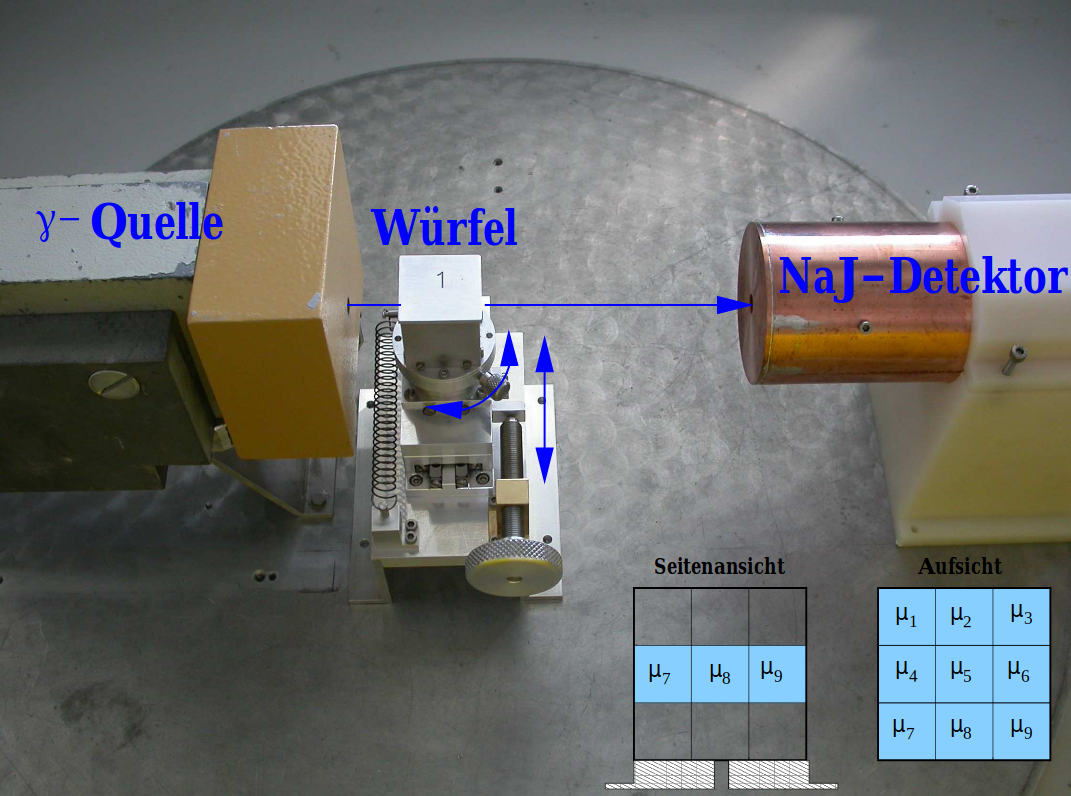
\includegraphics[width=\textwidth]{content/pics/Aufbau.png}
    \caption{Versuchsaufbau, \\aus \cite{anleitung}.}
    \label{abb:1}
  \end{minipage}
\end{figure}


\subsection{Versuchsdurchführung}
Zu Beginn wird ohne Würfel $I_{0}$ bestimmt und das Spektrum der Quelle aufgenommen.
Anschließend werden zwei Würfel bekannter und ein Würfel unbekannter Zusammensetzung
vermessen.
Dabei werden die in Abbildung \ref{abb:2} dargestellten Projektionen verwendet,
sodass die Würfelgeometrie durch Matrix \eqref{eq:3} beschrieben wird.
Es wird jeweils die mittlere der drei Schichten entlang der $z$-Achse der Würfel genutzt.

\begin{figure}[h!]
    \centering
    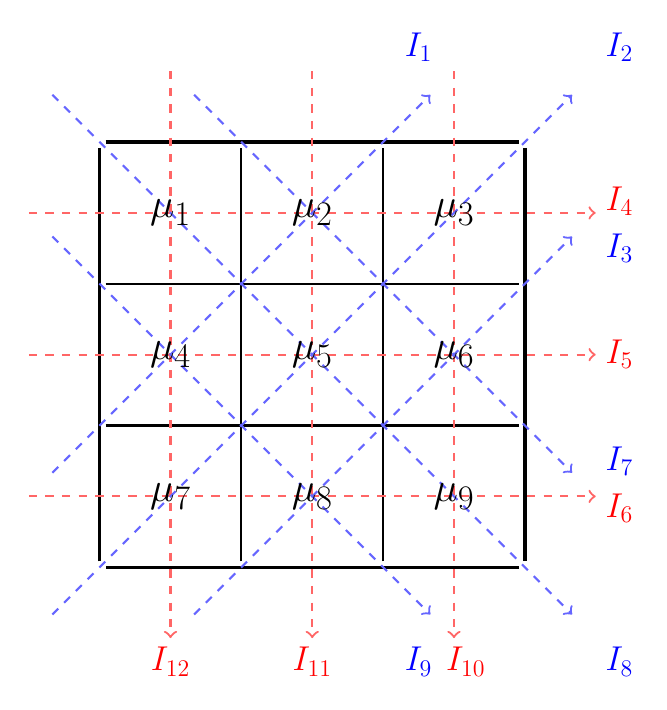
\begin{tikzpicture}[scale=0.6, every node/.style={scale=0.6}]
  % Kästchen
  \node (A1) at (0,0) {};
  \node (B1) at (0,3) {};
  \node (C1) at (0,6) {};
  \node (D1) at (0,9) {};
  \node (A2) at (3,0) {};
  \node (B2) at (3,3) {};
  \node (C2) at (3,6) {};
  \node (D2) at (3,9) {};
  \node (A3) at (6,0) {};
  \node (B3) at (6,3) {};
  \node (C3) at (6,6) {};
  \node (D3) at (6,9) {};
  \node (A4) at (9,0) {};
  \node (B4) at (9,3) {};
  \node (C4) at (9,6) {};
  \node (D4) at (9,9) {};

  \node (E1) at (0,0) {};
  \node (E2) at (0,9) {};
  \node (E3) at (9,9) {};
  \node (E4) at (9,0) {};


  % Umrandung
  \draw[very thick] (E1) to (E2) to (E3) to (E4) to (E1);
  \draw[thick] (B1) to (B4);
  \draw[thick] (C1) to (C4);
  \draw[thick] (A2) to (D2);
  \draw[thick] (A3) to (D3);

  % gerade Projektionen
  \draw[->, red!60, thick, dashed] (-1.5, 7.5) to (10.5, 7.5);
  \draw[->, red!60, thick, dashed] (-1.5, 4.5) to (10.5, 4.5);
  \draw[->, red!60, thick, dashed] (-1.5, 1.5) to (10.5, 1.5);

  \draw[->, red!60, thick, dashed] (1.5, 10.5) to (1.5, -1.5);
  \draw[->, red!60, thick, dashed] (4.5, 10.5) to (4.5, -1.5);
  \draw[->, red!60, thick, dashed] (7.5, 10.5) to (7.5, -1.5);

  % quere Projektionen
  \draw[->, blue!60, thick, dashed] (-1, -1) to (10, 10);
  \draw[->, blue!60, thick, dashed] (-1, 2) to (7, 10);
  \draw[->, blue!60, thick, dashed] (2, -1) to (10, 7);

  \draw[->, blue!60, thick, dashed] (2, 10) to (10, 2);
  \draw[->, blue!60, thick, dashed] (-1, 10) to (10, -1);
  \draw[->, blue!60, thick, dashed] (-1, 7) to (7, -1);

  % Erklärungsnodes
  \node [blue] at (6.75, 11) {\huge$I_{1}$};
  \node [blue] at (11, 11) {\huge$I_{2}$};
  \node [red] at (11, 7.75) {\huge$I_{4}$};
  \node [blue] at (11, 6.75) {\huge$I_{3}$};
  \node [red] at (11, 4.5) {\huge$I_{5}$};
  \node [blue] at (11, 2.25) {\huge$I_{7}$};
  \node [red] at (11, 1.25) {\huge$I_{6}$};
  \node [blue] at (11, -2) {\huge$I_{8}$};
  \node [red] at (7.75, -2) {\huge$I_{10}$};
  \node [blue] at (6.75, -2) {\huge$I_{9}$};
  \node [red] at (1.5, -2) {\huge$I_{12}$};
  \node [red] at (4.5, -2) {\huge$I_{11}$};

  %mu's
  \node at (1.5, 7.5) {\Huge$\mu_{1}$};
  \node at (4.5, 7.5) {\Huge$\mu_{2}$};
  \node at (7.5, 7.5) {\Huge$\mu_{3}$};

  \node at (1.5, 4.5) {\Huge$\mu_{4}$};
  \node at (4.5, 4.5) {\Huge$\mu_{5}$};
  \node at (7.5, 4.5) {\Huge$\mu_{6}$};

  \node at (1.5, 1.5) {\Huge$\mu_{7}$};
  \node at (4.5, 1.5) {\Huge$\mu_{8}$};
  \node at (7.5, 1.5) {\Huge$\mu_{9}$};
\end{tikzpicture}

    \caption{Verwendete Projektionen.}
    \label{abb:2}
\end{figure}

\begin{equation}
  \label{eq:3}
    \mathbf{A} =
    \begin{pmatrix}
      0 & \sqrt{2} & 0 & \sqrt{2} & 0 & 0 & 0 & 0 & 0\\
      0 & 0 & \sqrt{2} & 0 & \sqrt{2} & 0 & \sqrt{2} & 0 & 0\\
      0 & 0 & 0 & 0 & 0 & \sqrt{2} & 0 & \sqrt{2} & 0\\
      1 & 1 & 1 & 0 & 0 & 0 & 0 & 0 & 0\\
      0 & 0 & 0 & 1 & 1 & 1 & 0 & 0 & 0\\
      0 & 0 & 0 & 0 & 0 & 0 & 1 & 1 & 1\\
      0 & \sqrt{2} & 0 & 0 & 0 & \sqrt{2} & 0 & 0 & 0\\
      \sqrt{2} & 0 & 0 & 0 & \sqrt{2} & 0 & 0 & 0 & \sqrt{2}\\
      0 & 0 & 0 & \sqrt{2} & 0 & 0 & 0 & \sqrt{2} & 0\\
      0 & 0 & 1 & 0 & 0 & 1 & 0 & 0 & 1\\
      0 & 1 & 0 & 0 & 1 & 0 & 0 & 1 & 0\\
      1 & 0 & 0 & 1 & 0 & 0 & 1 & 0 & 0
    \end{pmatrix}
 \end{equation}
